\section{Security of Connect IQ store}
\subsection{Preliminary analysis}
Application allows the users to download third party apps to the watch.
The user can select an app to install it.

Notes:
\begin{itemize}
    \item the phone downloads the app
    \item sends it to the watch via BT
\end{itemize}

As the analysis of the Android application was not the main focus of the report, it does not go very deep.
However, it was necessary to have a basic understanding of the app to be able to analyze the communication between the watch and the phone.
This is described in the section~\ref{subsec:communication-watch-phone}.

\subsection{App decompilation}
I decompiled the app with JADX. The app is obfuscated.

I couldn't find any code that would be responsible for checking the certificate of the downloaded app.
I was looking for keywords such as the library that was used during a build process, SHA1, RSA\@.

Probably there is not much of a point to check the certificate on the phone, assuming that the watch is doing it.

I didn't manage to find the code responsible for downloading the app.
\subsection{Static analysis}

\subsection{Sniffing the traffic}
To analyze the network security, I tried to sniff the traffic between the phone and Garmin servers.
I decided to use mitmproxy\footnote{\url{https://mitmproxy.org/}}.
When dynamically analyzing the app, there are two opitons.
Either use an emulator or a real device.
Emulator usually offers more flexibility and is easier to manipulate.
However, it does not have access to Bluetooth, which is necessary to test the app.
For this reason, I used a real device.
- linux hotspot + mitmproxy - problem with certificates.
Two options to solve the problem:
- Rooted phone
- Modify the app

The minimum supported Android version is 7.
Those versions require root access to add certificates supported by applications.
Another option is to modify the app to accept user added certificates.

\subsubsection*{Attempt 1 - Android Unpinner}
Use Android Unpinner - https://github.com/mitmproxy/android-unpinner

The app starts when connected to mitmproxy.
However, when trying to log in, it goes back to the welcome screen.
**Not possible to log in**.

\subsubsection*{Attempt 2 — manually modify the apk and sign again}

Using Apktool(https://apktool.org/) to unpack the app, modify, and pack again, align zip file and sign with a debug key.

After installing the app, there are some errors with missing resources.
I did not investigate it further.

\subsubsection*{Attempt 3 — only resign the app.}
Just resigning the app with a debug key.
The app starts, but when trying to log in it seems to work the same as the app from the attempt \#1.

\subsubsection*{Attempt 4 — use rooted phone}
Short description about the root

\subsection{Network security,}
Based on the traffic that went through mitmproxy:

Used domains:
- `sso.garmin.com` - Qualys SSl Labs analysis: **grade B**
- server supports **TLS 1.1**
- `diauth.garmin.com` - Qualys SSl Labs analysis: **grade A**

\begin{figure}[h]
    \centering
    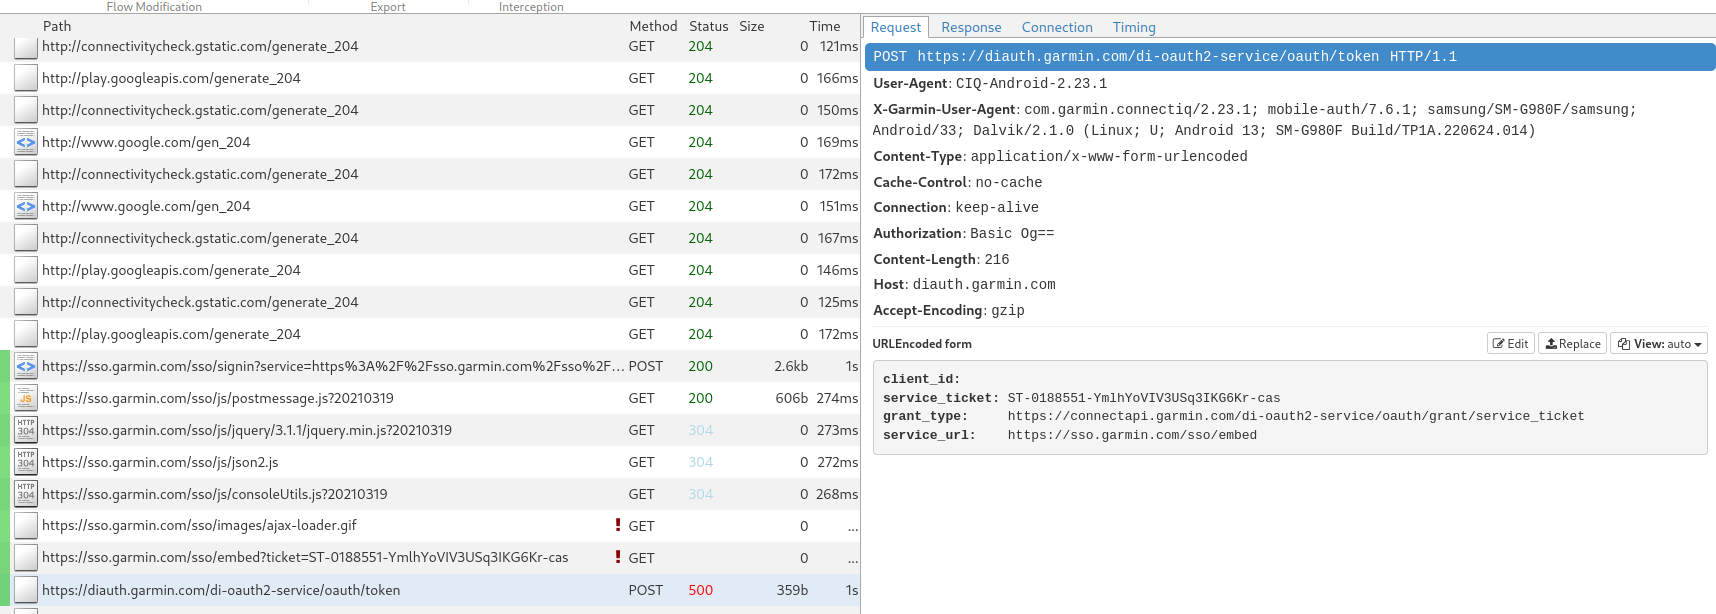
\includegraphics[width=1\linewidth]{../../images/mitmproxy unpinner}
    \caption{Sniffed traffic}
    \label{fig:mitmproxy-unpinner}
\end{figure}

\subsection{App sideloading}
- can we install an app that is not signed up by the store?
- app signed up only by the developer can be install through the cable, but not through the store
- the watch is probably checking the certificate
- it suggests that the Bluetooth API for app installation requires the app to be signed by the store - good thing
